\RequirePackage{fix-cm}
%
\RequirePackage{amsmath}



%\documentclass{svjour3}                     % onecolumn (standard format)
%\documentclass[smallcondensed]{svjour3}     % onecolumn (ditto)
%\documentclass[smallextended]{svjour3}       % onecolumn (second format)
% \documentclass[twocolumn]{svjour3}          % twocolumn
%\documentclass[letterpaper, 12pt, twocolumn]{article}
\documentclass{article}
\usepackage[cm]{fullpage}
%\usepackage[margin=1in]{geometry}
\usepackage{amssymb}
\usepackage{graphicx}
\usepackage[utf8]{inputenc}
\usepackage{indentfirst}
%\usepackage{physics}
\newcommand{\me}{\mathrm{e}}
\usepackage{amsmath}

%\usepackage[monochrome]{color}

%\usepackage[round]{natbib}
%\usepackage{apacite}
\usepackage{url}


\PassOptionsToPackage{monochrome}{xcolor}

% For the flow charts
\usepackage{tikz}
\usetikzlibrary{external}
\tikzexternalize

\usetikzlibrary{shapes.geometric, arrows, calc, positioning}
\tikzstyle{startstop} = [rectangle, thick, rounded corners=2.5mm, minimum width=2cm, minimum height=5mm,text centered, draw=black]
\tikzstyle{io} = [trapezium, thick, trapezium left angle=70, trapezium right angle=110, text width=3.75cm, minimum height=0.5cm, text centered, draw=black]
\tikzstyle{process} = [rectangle, thick, minimum width=2.5cm, text width=4cm, minimum height=0.5cm, text centered, draw=black]
\tikzstyle{decision} = [diamond, thick, minimum width=3cm, minimum height=1cm, text centered, draw=black]
\tikzstyle{dottedbox} = [rectangle, dotted, thick, minimum width=2.5cm, text width=2.8cm, minimum height=0.5cm, text centered, draw=black]
\tikzstyle{arrow} = [thick,->,>=stealth]
\tikzstyle{dottedarrow} = [thick, dotted,->,>=stealth]





\usepackage{pgfplots}
\usepgfplotslibrary{patchplots}
\pgfplotsset{compat=newest, samples=065} %Set this value to 65 for the final version
%\usepgfplotslibrary{dateplot} 


%\providecommand{\keywords}[1]{\textbf{\textit{Index terms---}} #1}

%\journalname{Journal of Science Education and Technology}

\begin{document}


\title{Algorithm to generate multi-factorial experiments to teach experimental design%\thanks{Grants or other notes
%about the article that should go on the front page should be
%placed here. General acknowledgments should be placed at the end of the article.}
}
%\subtitle{Do you have a subtitle?\\ If so, write it here}
%\titlerunning{Short form of title}        % if too long for running head
\author{A.C.~Delgado-Chavez  \and
        N.~Balagurusamy \and
        R.~Narayanasamy \and
        S.~K.~Gadi
}
%\authorrunning{Short form of author list} % if too long for running head
% The correct dates will be entered by the editor
\begin{figure}
	\centering
	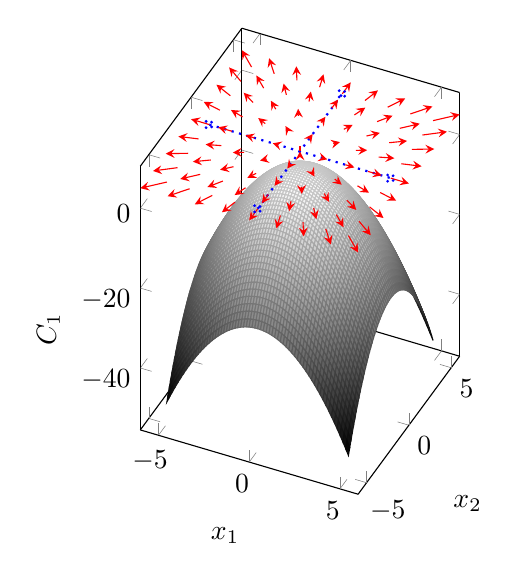
\begin{tikzpicture}
		\begin{axis}[
			width=0.465\textwidth,	
			height = 7.5cm,
			colormap/blackwhite,
			xlabel=$x_1$,
			ylabel=$x_2$,
			zlabel=$C_1$,
			]
			\addplot3[
			surf,
			%samples=10,
			domain=-5:5,
			]
			{-x^2-y^2};
			\addplot3 [blue, dotted, thick, mark=x] coordinates{(-5,0,5) (5,0,5)};
			\addplot3 [blue, dotted, thick, mark=x] coordinates{(0,-5,5) (0,5,5)};
			\addplot3[red,/pgfplots/quiver,
			quiver/u=2*x,
			quiver/v=2*y,
			quiver/w=0,
			quiver/scale arrows=0.1,
			-stealth,samples=9,
			domain=-5:5,
			] {5};			
		\end{axis}
	\end{tikzpicture}
	\caption{Two variable quadratic function $C_1(x_1, x_2)$.}
	\label{Fig:TwoVariablePolynomial}
\end{figure}



\begin{figure}
	\centering
	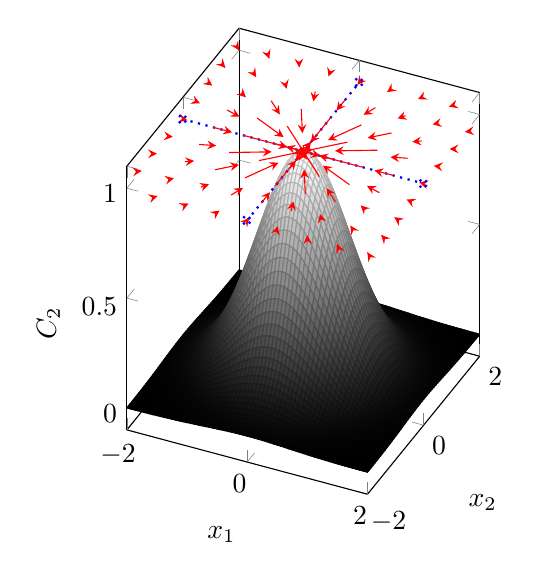
\begin{tikzpicture}
	\begin{axis}[
		width=0.50\textwidth,	
		height = 7.5cm,
		colormap/blackwhite,
		xlabel=$x_1$,
		ylabel=$x_2$,
		zlabel=$C_2$,
		]
		\addplot3[
		surf,
		%samples = 10,
		domain=-2:2,
		]
		{exp(-x^2-y^2)};
		\addplot3 [blue, dotted, thick, mark=x]coordinates {(-2,0,1) (2,0,1)};
		\addplot3 [blue, dotted, thick, mark=x] coordinates {(0,-2,1) (0,2,1)};
		\addplot3[red,/pgfplots/quiver,
		quiver/u=-2*x*exp(-x^2-y^2),
		quiver/v=-2*y*exp(-x^2-y^2),
		quiver/w=0,
		quiver/scale arrows=1,
		-stealth,samples=9,
		domain=-2:2,
		] {1};		
	\end{axis}
	\end{tikzpicture}
	\caption{Two variable Gaussian function $C_2(x_1, x_2)$.}
	\label{Fig:TwoVarGaussian}
\end{figure}



\begin{figure}
	\centering
	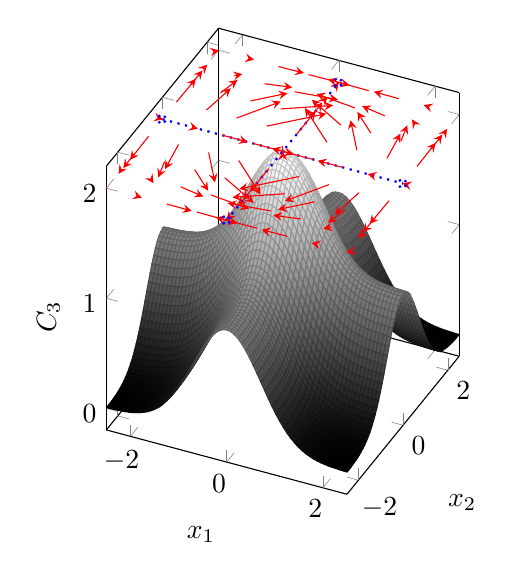
\begin{tikzpicture}
	\begin{axis}[
		width=0.50\textwidth,	
		height = 7.5cm,
		colormap/blackwhite,
		xlabel=$x_1$,
		ylabel=$x_2$,
		zlabel=$C_3$,
		]
		\addplot3[
		surf,
		%samples = 50,
		domain=-2.5:2.5,
		]
		{exp(-x^2)+exp(-y^2)};
			\addplot3 [blue, dotted, thick, mark=x] coordinates{(-2.5,0,2) (2.5,0,2)};
		\addplot3 [blue, dotted, thick, mark=x] coordinates{(0,-2.5,2) (0,2.5,2)};
		\addplot3[red,/pgfplots/quiver,
			quiver/u=-2*x*exp(-x^2),
			quiver/v=2*y*exp(-y^2),
			quiver/w=0,
			quiver/scale arrows=1,
			-stealth,samples=9,
			domain=-2.5:2.5,
			] {2};			
	\end{axis}
	\end{tikzpicture}	
	\caption{Modified version of Gaussian function $C_3(x_1, x_2)$.}
	\label{Fig:2GussianFunctionModified}
\end{figure}


\begin{figure}
	\centering
	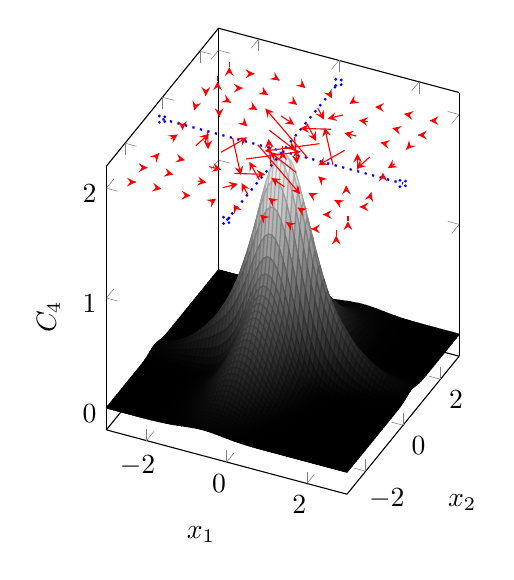
\begin{tikzpicture}
	\begin{axis}[
		width=0.50\textwidth,	
		height = 7.5cm,
		colormap/blackwhite,
		xlabel=$x_1$,
		ylabel=$x_2$,
		zlabel=$C_4$,
		]
		\addplot3[
		surf,
		%samples = 50,
		domain=-3:3,
		]
		{(
				 exp(-( 0.448*x + 0.308*y )^2)
			)*(  exp(-( 0.308*x + 0.338*y )^2)
			)*(( exp(-( 1.329*x - 0.493*y )^2)
			)+(  exp(-( -0.493*x + 2.761*y )^2)
			))};
			\addplot3 [blue, dotted, thick, mark=x] coordinates{(-3,0,2) (3,0,2)};
			\addplot3 [blue, dotted, thick, mark=x] coordinates{(0,-3,2) (0,3,2)};
			\addplot3[red,/pgfplots/quiver,
			quiver/u=-exp(-((56*x)/125 + (77*y)/250)^2)*exp(-((77*x)/250 + (169*y)/500)^2)*(exp(-((493*x)/1000 - (2761*y)/1000)^2)*((243049*x)/500000 - (1361173*y)/500000) + exp(-((1329*x)/1000 - (493*y)/1000)^2)*((1766241*x)/500000 - (655197*y)/500000)) - exp(-((56*x)/125 + (77*y)/250)^2)*exp(-((77*x)/250 + (169*y)/500)^2)*((6272*x)/15625 + (4312*y)/15625)*(exp(-((1329*x)/1000 - (493*y)/1000)^2) + exp(-((493*x)/1000 - (2761*y)/1000)^2)) - exp(-((56*x)/125 + (77*y)/250)^2)*exp(-((77*x)/250 + (169*y)/500)^2)*((5929*x)/31250 + (13013*y)/62500)*(exp(-((1329*x)/1000 - (493*y)/1000)^2) + exp(-((493*x)/1000 - (2761*y)/1000)^2)),
			quiver/v= exp(-((56*x)/125 + (77*y)/250)^2)*exp(-((77*x)/250 + (169*y)/500)^2)*(exp(-((1329*x)/1000 - (493*y)/1000)^2)*((655197*x)/500000 - (243049*y)/500000) + exp(-((493*x)/1000 - (2761*y)/1000)^2)*((1361173*x)/500000 - (7623121*y)/500000)) - exp(-((56*x)/125 + (77*y)/250)^2)*exp(-((77*x)/250 + (169*y)/500)^2)*((4312*x)/15625 + (5929*y)/31250)*(exp(-((1329*x)/1000 - (493*y)/1000)^2) + exp(-((493*x)/1000 - (2761*y)/1000)^2)) - exp(-((56*x)/125 + (77*y)/250)^2)*exp(-((77*x)/250 + (169*y)/500)^2)*((13013*x)/62500 + (28561*y)/125000)*(exp(-((1329*x)/1000 - (493*y)/1000)^2) + exp(-((493*x)/1000 - (2761*y)/1000)^2)),
			quiver/w=0,
			quiver/scale arrows=1,
			-stealth,samples=9,
			domain=-2.5:2.5,
			] {2};			
	\end{axis}
	\end{tikzpicture}
	\caption[Proposed function 1]{The proposed function $C_4(x_1, x_2)$ for $P=\left[ \begin{matrix}
		\text{0}\text{.448} & \text{0}\text{.308}  \\
		\text{0}\text{.308} & \text{0}\text{.338}  \\
		\end{matrix} \right]$
		and $Q=\left[ \begin{matrix}
		\text{1}\text{.329} & \text{-0}\text{.493}  \\
		\text{-0}\text{.493} & \text{2}\text{.761}  \\
		\end{matrix} \right]$.}
	\label{Fig:TwoVarNovelFunc}
\end{figure}

\begin{figure}
	\centering
	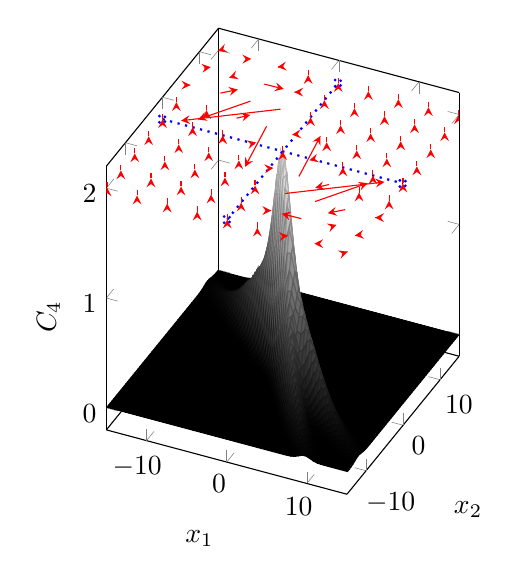
\begin{tikzpicture}
	\begin{axis}[
	width=0.50\textwidth,	
	height = 7.5cm,
	colormap/blackwhite,
	xlabel=$x_1$,
	ylabel=$x_2$,
	zlabel=$C_4$,
	]
	\addplot3[
	surf,
	%samples = 50,
	domain=-15:15,
	]
	{(
			 exp(-( 0.1*x + 0.0*y )^2)
		)*(  exp(-( 0.0*x + 0.1*y )^2)
		)*(( exp(-( 0.979*x + 0.636*y )^2)
		)+(  exp(-( 0.636*x + 0.773*y )^2)
		))};
		\addplot3 [blue, dotted, thick, mark=x] coordinates{(-15,0,2) (15,0,2)};
		\addplot3 [blue, dotted, thick, mark=x] coordinates{(0,-15,2) (0,15,2)};
		\addplot3[red,/pgfplots/quiver,
			quiver/u=- exp(-x^2/100)*exp(-y^2/100)*(exp(-((159*x)/250 + (773*y)/1000)^2)*((25281*x)/31250 + (122907*y)/125000) + exp(-((979*x)/1000 + (159*y)/250)^2)*((958441*x)/500000 + (155661*y)/125000)) - (x*exp(-x^2/100)*exp(-y^2/100)*(exp(-((159*x)/250 + (773*y)/1000)^2) + exp(-((979*x)/1000 + (159*y)/250)^2)))/50,
			quiver/v=- exp(-x^2/100)*exp(-y^2/100)*(exp(-((979*x)/1000 + (159*y)/250)^2)*((155661*x)/125000 + (25281*y)/31250) + exp(-((159*x)/250 + (773*y)/1000)^2)*((122907*x)/125000 + (597529*y)/500000)) - (y*exp(-x^2/100)*exp(-y^2/100)*(exp(-((159*x)/250 + (773*y)/1000)^2) + exp(-((979*x)/1000 + (159*y)/250)^2)))/50,
			quiver/w=0,
			quiver/scale arrows=30,
			-stealth,samples=9,
			domain=-15:15,
			] {2};			
	\end{axis}
	\end{tikzpicture}
	\caption[Proposed function 1]{The proposed function $C_4(x_1, x_2)$ for $P=\left[ \begin{matrix}
		0.1 & 0  \\
		0 & 0.1  \\
		\end{matrix} \right]$, $Q=\left[ \begin{matrix}
		\text{0}\text{.979} & \text{0}\text{.636}  \\
		\text{0}\text{.636} & \text{0}\text{.773}  \\
		\end{matrix} \right]$
		.}
	\label{Fig:TwoVarNovelFunc}
\end{figure}

\pagebreak
\begin{figure}
	\centering
	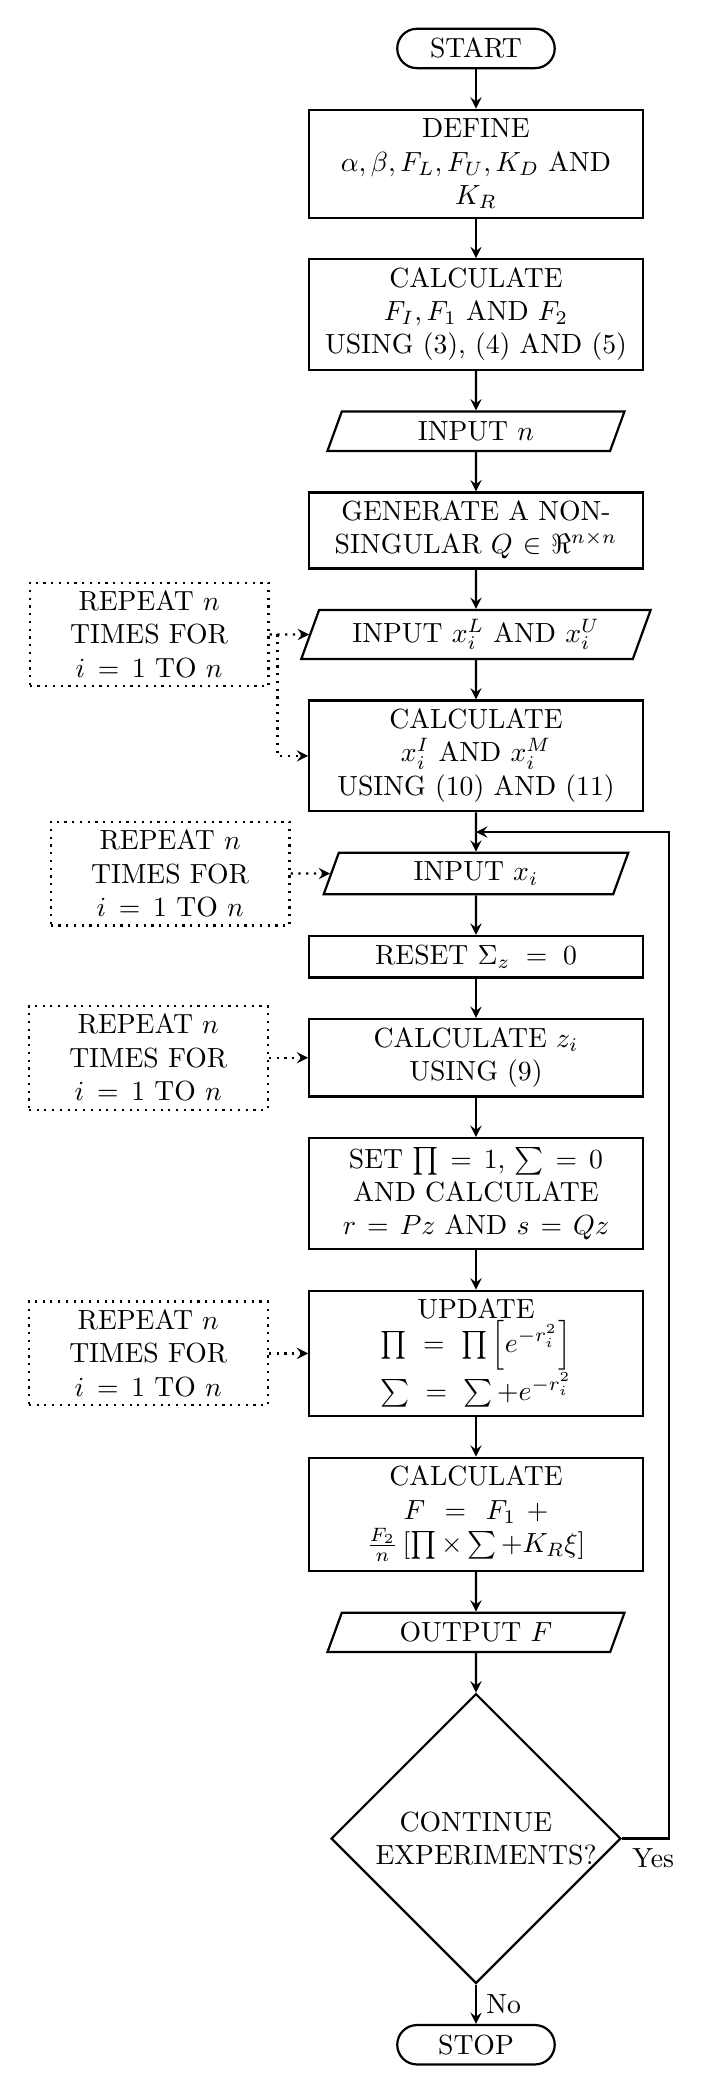
\begin{tikzpicture}[node distance = 5mm, auto]
		\node (Start) [startstop] {START};
		\node (Define) [process, below = of Start] {DEFINE $\alpha, \beta, F_L, F_U, K_D$~AND $K_R$};
		\node (Calculate01) [process, below =of Define] {CALCULATE\\$F_I, F_1$ AND $F_2$\\USING (3), (4) AND (5)};
		\node (Input01) [io, below = of Calculate01, text width=3cm] {INPUT $n$};
		\node (Calculate01a) [process, below = of Input01] {GENERATE A NONSINGULAR $Q\in \Re^{n\times n}$};
		\node (Input02) [io, below = of Calculate01a] {INPUT $x_i^L$~AND~$x_i^U$};
		\node (Calculate02) [process, below = of Input02] {CALCULATE\\$x_i^I$ AND $x_i^M$\\USING (10) AND (11)};
		\node (Input03) [io, below = of Calculate02, text width=3.25cm] {INPUT $x_i$};
		\node (Calculate03) [process, below = of Input03] {RESET $\Sigma_z=0$};
		\node (Calculate04) [process, below = of Calculate03] {CALCULATE $z_i$\\ USING (9)};
		\node (Calculate05) [process, below = of Calculate04] {SET $\prod=1$, $\sum = 0$ \\AND CALCULATE \\ $r=Pz$ AND $s=Qz$};
		\node (Calculate06) [process, below = of Calculate05] {UPDATE\\ $\prod = \prod \left[e^{-r_i^2}\right]$\\$\sum=\sum + e^{-r_i^2}$};
		\node (Calculate07) [process, below = of Calculate06] {CALCULATE \\ $F=F_1+\frac{F_2}{n}\left[\prod \times \sum + K_R\xi\right]$};
		\node (Output03) [io, below = of Calculate07, text width=3cm] {OUTPUT $F$};
		\node (Decision01) [decision, below = of Output03, text width=2.55cm] {CONTINUE\\EXPERIMENTS?};
		\node (Stop) [startstop, below = of Decision01] {STOP};

		\node (ForBox01) [dottedbox, left = of Input02, left = 5mm] {REPEAT $n$ TIMES FOR $i=1$ TO $n$};
		%\node (ForBox02) [dottedbox, left of=Calculate02, left = 2.25cm] {REPEAT $n$ TIMES FOR $i=1$ TO $n$};
		\node (ForBox03) [dottedbox, left = of Input03, left = 5mm] {REPEAT $n$ TIMES FOR $i=1$ TO $n$};
		\node (ForBox04) [dottedbox, left = of Calculate04, left = 5mm] {REPEAT $n$ TIMES FOR $i=1$ TO $n$};
		\node (ForBox05) [dottedbox, left = of Calculate06, left = 5mm] {REPEAT $n$ TIMES FOR $i=1$ TO $n$};

 		%\node (stop) [startstop, below of=calculate1, below = 0mm] {STOP};
		\draw [arrow] (Start) -- (Define);
		\draw [arrow] (Define) -- (Calculate01);
		\draw [arrow] (Calculate01) -- (Input01);
		\draw [arrow] (Input01) -- (Calculate01a);
		\draw [arrow] (Calculate01a) -- (Input02);
		\draw [arrow] (Input02) -- (Calculate02);
		\draw [arrow] (Calculate02) -- (Input03);
		\draw [arrow] (Input03) -- (Calculate03);
		\draw [arrow] (Calculate03) -- (Calculate04);
		\draw [arrow] (Calculate04) -- (Calculate05);
		\draw [arrow] (Calculate05) -- (Calculate06);
		\draw [arrow] (Calculate06) -- (Calculate07);
		\draw [arrow] (Calculate07) -- (Output03);
		\draw [arrow] (Output03) -- (Decision01);
		\draw [arrow] (Decision01) -- node[anchor=west]{No}(Stop);
		\draw [arrow] ($ (Decision01.east) $)node[anchor=north west]{Yes}  -- ++(0.6,0.00) |- ($ (Input03.north) + (0mm,2.5mm) $);

		\draw [dottedarrow] (ForBox01) -- (Input02);
		%\draw [dottedarrow] (ForBox02) -- (Calculate02);
		\draw [dottedarrow] ($(ForBox01.east) + (1mm,0mm)$) |- (Calculate02);
		\draw [dottedarrow] (ForBox03) -- (Input03);
		\draw [dottedarrow] (ForBox04) -- (Calculate04);
		\draw [dottedarrow] (ForBox05) -- (Calculate06);
	\end{tikzpicture}
	\caption{Flowchart of the proposed algorithm}
	\label{Fig:AlgorithmInFlowchart}
\end{figure}


\begin{figure}
	\centering
	\includegraphics[width=\textwidth]{Ver011-figure9}
	\caption{Screenshot of the application.}
	\label{Fig:TwoVarNovelFunc5}
\end{figure}


\begin{figure}
	\centering
	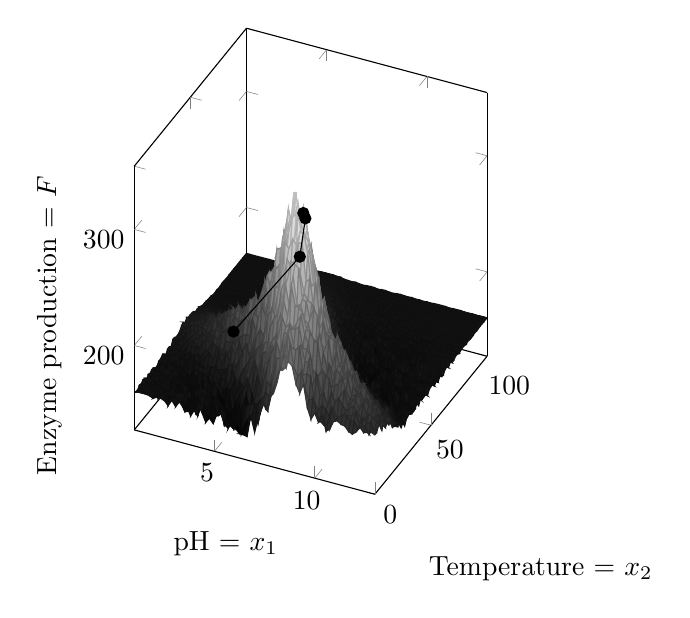
\begin{tikzpicture}
	\begin{axis}[
	width=0.50\textwidth,	
	height = 7.5cm,
	colormap/blackwhite,
	xlabel={pH = $x_1$},
	ylabel={Temperature = $x_2$},
	zlabel={Enzyme production = $F$},
	]
	\addplot3[
	surf,
	%samples = 50,
	domain = 1:13,
	domain y = 0:100,
	]
	{160.49815877303246 + 167.90759039534183/2*(
		exp(-(5/12*(x - 7.784)*0.5)^2)*exp(-(5/100*(y - 23.606)*0.5)^2)
		* ( exp(-(2.128*5/12*(x - 7.784) + 0.675*5/100*(y - 23.606))^2)
		+ exp(-(0.675*5/12*(x - 7.784) + 1.452*5/100*(y - 23.606))^2)
		+ (rand-0.5)*2*0.1
		)
	};
	%{193.043 + 275.866/2 * exp(-(5/100*(x-25.291) + 0.475*sin( 5/100*(x-25.291) + 5/2*(y-0.356))) * exp(-(5/2*(y-0.356) + 0.475*sin( 5/100*(x-25.291) + 5/2*(y-0.356)))};
	\addplot3 [color= black,mark=*,] coordinates {
		(4.375, 28.125, 194.1394)
		(7.036, 39.667, 257.2037)
		(8.209, 23.667, 314.6647)
		(8.150, 22.880, 319.9692)
	};
	\end{axis}
	\end{tikzpicture}
	\caption{Surface plot of $F$ with the constants given in Section~6 superimposed with the RSM results.}
	\label{Fig:TwoVarNovelFunc4}
\end{figure}


\begin{figure}
	\centering
	\begin{tikzpicture}
	\begin{axis}
		[
		colormap/blackwhite,
		width=0.50\textwidth,	
		xlabel={pH = $x_1$},
		ylabel={Temperature = $x_2$},
		zlabel={Enzyme production = $F$},
		view={0}{90}
		]
		\addplot3[contour gnuplot ={number=20,
			labels=false,
		},
		domain = 1:13,
		domain y = 0:100,
		%thick,
		]
		{160.49815877303246 + 167.90759039534183/2*(
			exp(-(5/12*(x - 7.784)*0.5)^2)*exp(-(5/100*(y - 23.606)*0.5)^2)
			+ exp(-(2.128*5/12*(x - 7.784) + 0.675*5/100*(y - 23.606))^2)
			+ exp(-(0.675*5/12*(x - 7.784) + 1.452*5/100*(y - 23.606))^2)
			)
		};
		\addplot3 [color= black,mark=*,] coordinates {
		(4.375, 28.125, 194.1394)
		(7.036, 39.667, 257.2037)
		(8.209, 23.667, 314.6647)
		(8.150, 22.880, 319.9692)
		};
	\end{axis}
	\end{tikzpicture}
	\caption{Contour plot of $F$ with $K_R=0$ and the other constants given in Section~6 superimposed with the RSM results.}
	\label{Fig:Application2Variable}
\end{figure}





\begin{figure}
	\centering
	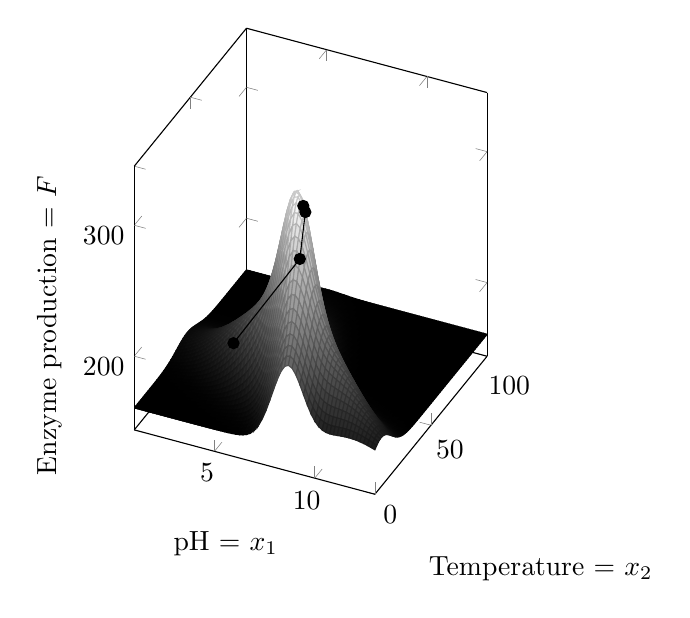
\begin{tikzpicture}
	\begin{axis}[
	colormap/blackwhite,
	width=0.50\textwidth,	
	height = 7.5cm,
	xlabel={pH = $x_1$},
	ylabel={Temperature = $x_2$},	
	zlabel={Enzyme production = $F$},
	]
	\addplot3[
	surf,
	%samples = 50,
		domain = 1:13,
		domain y = 0:100,
	]
	{160.49815877303246 + 167.90759039534183/2*(
		exp(-(5/12*(x - 7.784)*0.5)^2)*exp(-(5/100*(y - 23.606)*0.5)^2)
		* ( exp(-(2.128*5/12*(x - 7.784) + 0.675*5/100*(y - 23.606))^2)
		+ exp(-(0.675*5/12*(x - 7.784) + 1.452*5/100*(y - 23.606))^2)
		))
	};
		\addplot3 [color= black,mark=*,] coordinates {
		(4.375, 28.125, 194.1394)
		(7.036, 39.667, 257.2037)
		(8.209, 23.667, 314.6647)
		(8.150, 22.880, 319.9692)
	};
	%{193.043 + 275.866/2 * exp(-(5/100*(x-25.291) + 0.475*sin( 5/100*(x-25.291) + 5/2*(y-0.356))) * exp(-(5/2*(y-0.356) + 0.475*sin( 5/100*(x-25.291) + 5/2*(y-0.356)))};
%		\addplot3 [blue, dotted, thick, mark=x] coordinates{(7.784,1,328.406) (7.784,100,328.406)};
%		\addplot3 [blue, dotted, thick, mark=x] coordinates{(0,23.606,328.406) (13,23.606,328.406)};
%		\addplot3[red,/pgfplots/quiver,
%			quiver/u=- (5907723137008901*exp(-((5*x)/24 - 973/600)^2)*exp(-(y/40 - 11803/20000)^2)*(exp(-((9*x)/32 + (363*y)/5000 - 4878807/1250000)^2)*((81*x)/512 + (3267*y)/80000 - 43909263/20000000) + exp(-((133*x)/150 + (27*y)/800 - 9238219/1200000)^2)*((17689*x)/11250 + (1197*y)/20000 - 1228683127/90000000)))/70368744177664 - (5907723137008901*exp(-((5*x)/24 - 973/600)^2)*exp(-(y/40 - 11803/20000)^2)*((25*x)/288 - 973/1440)*(exp(-((9*x)/32 + (363*y)/5000 - 4878807/1250000)^2) + exp(-((133*x)/150 + (27*y)/800 - 9238219/1200000)^2)))/70368744177664,
%			quiver/v= - (5907723137008901*exp(-((5*x)/24 - 973/600)^2)*exp(-(y/40 - 11803/20000)^2)*(exp(-((133*x)/150 + (27*y)/800 - 9238219/1200000)^2)*((1197*x)/20000 + (729*y)/320000 - 83143971/160000000) + exp(-((9*x)/32 + (363*y)/5000 - 4878807/1250000)^2)*((3267*x)/80000 + (131769*y)/12500000 - 1771006941/3125000000)))/70368744177664 - (5907723137008901*exp(-((5*x)/24 - 973/600)^2)*exp(-(y/40 - 11803/20000)^2)*(y/800 - 11803/400000)*(exp(-((9*x)/32 + (363*y)/5000 - 4878807/1250000)^2) + exp(-((133*x)/150 + (27*y)/800 - 9238219/1200000)^2)))/70368744177664,
%			quiver/w=0,
%			quiver/scale arrows=.1,
%			-stealth,samples=9,
%			domain = 1:13,
%			domain y = 0:100,
%		] {325};			
	\end{axis}
	\end{tikzpicture}
	\caption{Surface plot of $F$ with $K_R=0$ and the other constants given in Section~6 superimposed with the RSM results.}
	\label{Fig:TwoVarNovelFunc6}
\end{figure}



%\bibliographystyle{apacite}%unsrtnat}
%\bibliographystyle{spbasic}      % basic style, author-year citations
%\bibliographystyle{spmpsci}      % mathematics and physical sciences
%\bibliographystyle{spphys}       % APS-like style for physics
%\bibliographystyle{ieeetr}
%\bibliography{refs}
\end{document}